%======================================================================
\section{Dinámica de las trayectorias: comparación entre formulaciones}\label{sec:trayectorias}
%======================================================================
\paragraph{Qué falta en las secciones anteriores.} Las tablas de las secciones
\ref{sec:desempeno} y \ref{sec:riesgo-formulaciones} resumen cada lazo cerrado en una cifra
(IAE, pico, probabilidad de cruce), y la figura~\ref{fig:syn-cl-compare} compara N2 con los
controladores de la tesis. Ninguna muestra si las \emph{formulaciones} del MPC (N1, N2, N3 y las
variantes de riesgo) producen trayectorias distintas, cuándo se separan ni por qué. Esta sección
lo hace con las trayectorias completas de la campaña F6: 50 realizaciones por familia, con
números aleatorios comunes, de modo que cada par de controladores ve exactamente la misma
planta, la misma fuga y las mismas fallas.

\paragraph{Cómo se mide.} Para dos controladores $A$ y $B$ en la misma realización se calcula
$\max_t|\mathrm{PCT}_A(t)-\mathrm{PCT}_B(t)|$, la mayor distancia entre sus trayectorias de
temperatura, y lo mismo con el caudal entregado. La PCT se registró con cuatro decimales, de
modo que diferencias bajo $10^{-4}$~K no se resuelven. Las cifras están en
\code{results/f6\_paper/trajectory\_distances.csv} y las figuras en
\code{python/make\_trajectory\_figures.py}.

\subsection{N1, N2 y N3 dan la misma trayectoria salvo en la familia extrema}

\begin{figure}[H]\centering
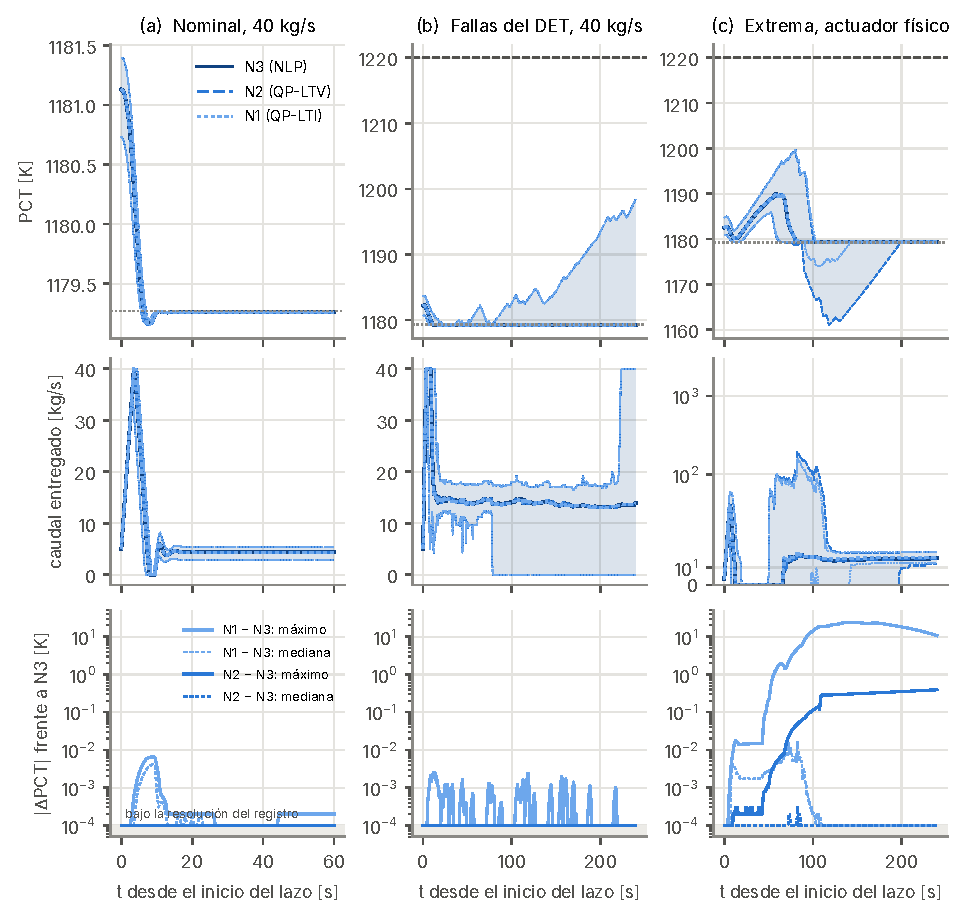
\includegraphics[width=\linewidth]{figures/traj_formulations.pdf}
\caption{N1, N2 y N3 en lazo cerrado, 50 realizaciones por familia. Fila superior: PCT
(mediana y banda 10--90\,\% de N3; las líneas finas son los bordes de la banda de N1 y N2).
Fila central: caudal entregado. Fila inferior: diferencia de PCT frente a N3, máxima y mediana
sobre las 50 realizaciones, en escala logarítmica; la franja gris está bajo la resolución del
registro. En la familia extrema el eje del caudal es lineal hasta 50~kg/s y logarítmico encima.}
\label{fig:traj-formulations}
\end{figure}

\begin{table}[H]\centering\small
\begin{tabularx}{\linewidth}{@{}l Y r r r r@{}}\toprule
Familia & Par & \multicolumn{3}{c}{$\max_t|\Delta\mathrm{PCT}|$ [K]} & Se separan\\
\cmidrule(lr){3-5}
& & mediana & p90 & máx. & ($>0.01$~K)\\\midrule
Nominal, bomba archivada & N1, N2 frente a N3 & $<10^{-4}$ & $<10^{-4}$ & $<10^{-4}$ & 0\,\%\\
Nominal, 40~kg/s & N2 frente a N3 & $<10^{-4}$ & $<10^{-4}$ & $<10^{-4}$ & 0\,\%\\
 & N1 frente a N3 & 0.0044 & 0.0060 & 0.0066 & 0\,\%\\
Fallas del DET, 40~kg/s & N2 frente a N3 & $<10^{-4}$ & $<10^{-4}$ & $<10^{-4}$ & 0\,\%\\
 & N1 frente a N3 & 0.0012 & 0.0021 & 0.0025 & 0\,\%\\
Extrema, actuador físico & N2 frente a N3 & 0.0068 & 0.14 & 0.39 & 40\,\%\\
 & N1 frente a N3 & \textbf{1.42} & \textbf{14.4} & \textbf{24.2} & 100\,\%\\\bottomrule
\end{tabularx}
\caption{Distancia entre las trayectorias de PCT de las formulaciones, 50 realizaciones por
fila. «Se separan»: fracción de realizaciones en que la distancia supera 0.01~K en algún
instante. En la familia extrema la separación empieza, en mediana, a los 63~s (N1) y a los 84~s
(N2), es decir, después de la falla del ACS.}
\label{tab:traj-dist}
\end{table}

\paragraph{Lectura.}
\begin{enumerate}
  \item \textbf{En el escenario de la tesis y con fallas del DET, la formulación no cambia la
        trayectoria.} N2 y N3 coinciden bajo la resolución del registro en las 100 realizaciones,
        y N1 se aparta a lo más 7~mK, cincuenta veces menos que la banda de asentamiento de
        0.30~K. Las tres fases de la dinámica (rampa hasta saturar, caída hacia la consigna con
        un pequeño sobrepaso y regulación con unos 4--15~kg/s) son las mismas para las tres
        formulaciones (figura~\ref{fig:traj-formulations}a--b). Es la versión en lazo cerrado
        del resultado en lazo abierto de la sección~\ref{sec:comparacion}: en esta región el
        modelo lineal es exacto a efectos prácticos.
  \item \textbf{En la familia extrema, N1 se separa de N3 y N2 no.} La distancia mediana N1--N3
        es de 1.4~K y llega a 24~K. N2 queda bajo 0.4~K en las 50 realizaciones. La separación
        aparece después de la falla, cuando la planta ha salido de la región en que se
        linealizó N1 (PCT de hasta 1206~K y caudales de cientos de kg/s). Como N2 relinealiza en
        cada consulta, sigue a N3.
\end{enumerate}

\subsection{Dónde y por qué se separa N1: la familia extrema}

\begin{figure}[H]\centering
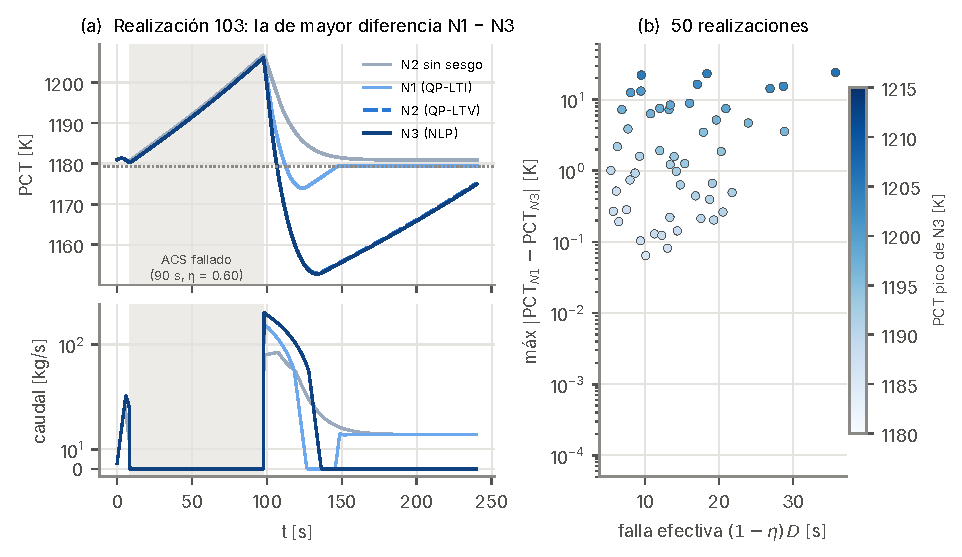
\includegraphics[width=\linewidth]{figures/traj_extreme_n1.pdf}
\caption{(a) La realización con mayor distancia N1--N3 (semilla 103): una falla de 90~s, con
el ACS a un 60\,\% de su capacidad al volver ($\eta=0.60$, desconocido para el MPC). Al
terminar la falla, N2 y N3 mandan 230~kg/s y sobre-enfrían hasta 1153~K; N1 manda 172~kg/s y
baja hasta 1174~K; N2 sin corrección de sesgo no sobre-enfría. (b) Distancia N1--N3 por
realización frente a la falla efectiva $(1-\eta)D$, coloreada por el pico de N3.}
\label{fig:traj-extreme}
\end{figure}

\noindent La figura~\ref{fig:traj-extreme} muestra el mecanismo. Durante la falla, la corrección
de sesgo absorbe el desajuste entre el ROM y la planta; al volver el ACS con una capacidad
reducida que el modelo no conoce, ese sesgo queda desactualizado y el MPC pide más caudal del
necesario. Las tres formulaciones reciben el mismo sesgo, pero N1 predice con otra ganancia
(la del punto de linealización) y por eso responde distinto. En la semilla 103 eso le favorece:
su IAE es de 1496~K\,s frente a 3510~K\,s de N3. En las 50 realizaciones, la diferencia mediana
de IAE entre N1 y N3 es de $-0.1$~K\,s y N1 es mejor en la mitad de ellas; el sobrepaso mínimo
mediano es de $+0.01$~K para N1 y de $-1.2$~K para N3. La correlación con la severidad de la
falla es débil ($r=0.31$ entre $\log|\Delta\mathrm{PCT}|$ y $(1-\eta)D$): la separación depende
de cómo se combinan la duración, $\eta$ y el sesgo de pronóstico, no de una sola variable.

\paragraph{Consecuencia.} Un mejor optimizador del P0 no da necesariamente una mejor
trayectoria cuando la planta tiene perturbaciones que el modelo no conoce. Las diferencias de la
familia extrema no vienen de que N1 resuelva peor el P0, sino de que el P0 mismo está mal
informado (sesgo desactualizado, $\eta$ desconocido). Por eso la certificación de optimalidad
(secciones~\ref{sec:auditoria} y~\ref{sec:f7}) responde a la pregunta
«¿resuelve el solver el problema que se le plantea?», y no a «¿es ese el problema correcto?».

\subsection{Las formulaciones de riesgo: pre-enfrían distinto, se calientan igual}

\begin{figure}[H]\centering
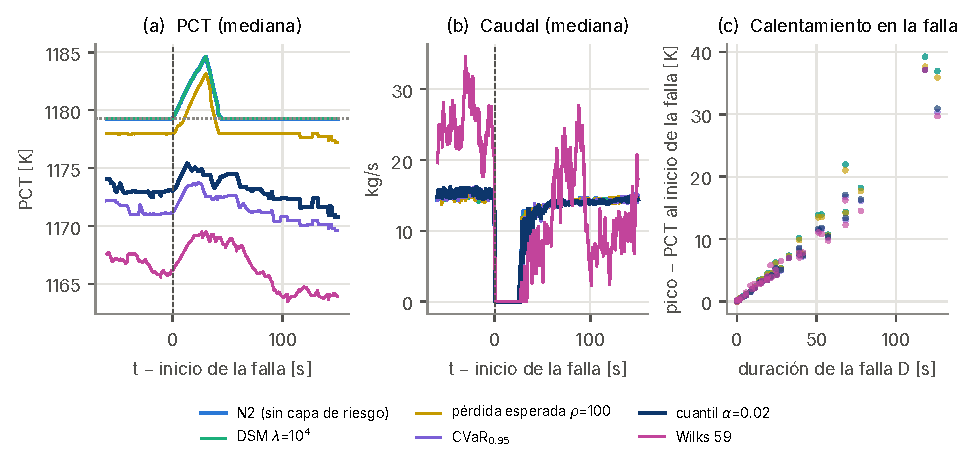
\includegraphics[width=\linewidth]{figures/traj_risk_dynamics.pdf}
\caption{Familia de fallas del DET (40~kg/s), 46 realizaciones con una sola falla, alineadas en
su inicio. (a) PCT mediana: cada formulación de riesgo entra a la falla con un margen distinto
bajo $y_{\rm ref}$. (b) Caudal mediano: cero durante la falla y luego la misma recuperación.
(c) Calentamiento del episodio (pico menos PCT al inicio) frente a la duración de la falla, sólo
para fallas que terminan antes del fin de la corrida: las seis formulaciones caen sobre la misma
curva $\Delta T(D)$.}
\label{fig:traj-risk}
\end{figure}

\begin{table}[H]\centering\small
\begin{tabularx}{\linewidth}{@{}Y r r r r@{}}\toprule
Formulación & Pre-enfr.\ [K] & Calent.\ [K] & Pico [K] & $\max_t|\Delta\mathrm{PCT}|$ frente a N2 [K]\\\midrule
N2 (sin capa de riesgo) & $-0.02$ & 5.8 & 1185.8 & ---\\
DSM $\lambda=10^4$ & $-0.02$ & 5.8 & 1185.8 & 0.020\\
Pérdida esperada $\rho=100$ & 1.3 & 5.7 & 1183.7 & 2.5\\
Cuantil $\alpha=0.02$ & 6.2 & 5.2 & 1179.0 & 8.7\\
CVaR$_{0.95}$ & 8.1 & 5.1 & 1177.9 & 9.9\\
Wilks 59 & 13.1 & 6.1 & 1172.9 & 18.4\\\bottomrule
\end{tabularx}
\caption{Medianas sobre las realizaciones con una falla. Pre-enfriamiento:
$y_{\rm ref}-\mathrm{PCT}$ al inicio de la falla. Calentamiento: pico del episodio menos la PCT
al inicio. Última columna: sobre las 50 realizaciones.}
\label{tab:traj-risk}
\end{table}

\noindent Las trayectorias confirman en lazo cerrado lo que la proposición~\ref{prop:margen}
predice. Cada formulación de riesgo actúa \emph{antes} de la falla, manteniendo la PCT un
margen bajo la consigna (de 1.3~K la pérdida esperada a 13~K Wilks). Durante la falla todas
quedan sin actuador y se calientan lo mismo para la misma duración (5.1--6.1~K en mediana;
figura~\ref{fig:traj-risk}c), porque el calentamiento depende de $D$ y no del controlador. El
pico es entonces el margen más un calentamiento común: las formulaciones se distinguen sólo por
el margen que eligen, que es la reducción a un margen de la proposición. Los estados
pre-enfriados se calientan algo más lento (5.1--5.2~K frente a 5.8~K), lo que es el lado seguro
del supuesto A1. Wilks, cuyo margen se sortea de nuevo en cada consulta, hace oscilar el caudal
antes de la falla (figura~\ref{fig:traj-risk}b), pero la misma oscilación no cambia el
calentamiento.

\subsection{Síntesis: qué cambia una trayectoria}

\begin{figure}[H]\centering
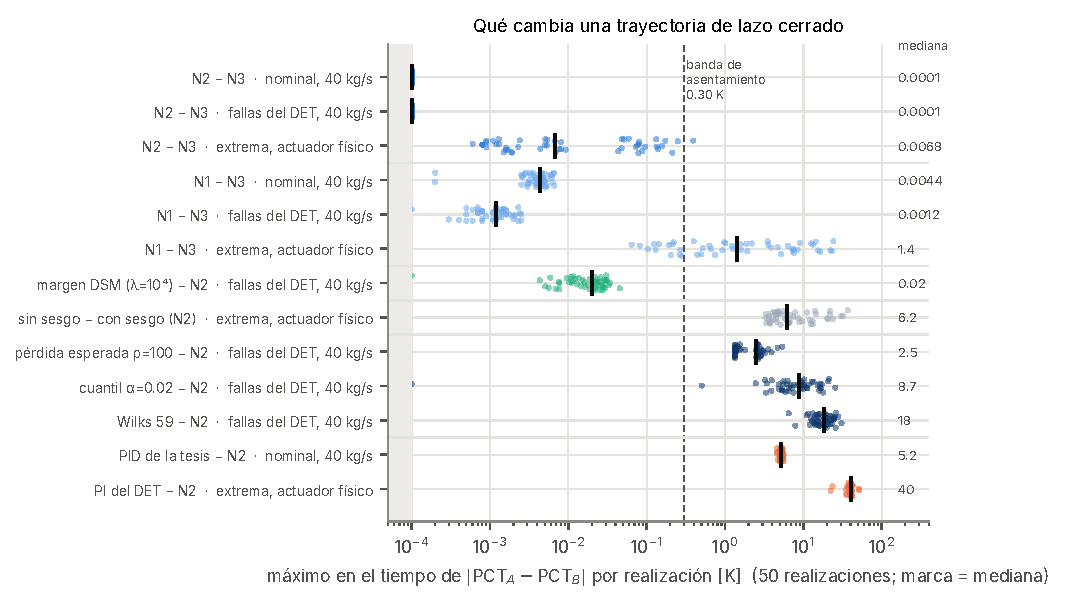
\includegraphics[width=\linewidth]{figures/traj_hierarchy.pdf}
\caption{Distancia entre trayectorias de PCT para cada comparación, una marca por realización
(50 por fila) y la mediana en negro. Escala logarítmica; la línea de trazos es la banda de
asentamiento de 0.30~K y la franja gris, la resolución del registro.}
\label{fig:traj-hierarchy}
\end{figure}

\noindent La figura~\ref{fig:traj-hierarchy} ordena las decisiones de diseño por cuánto mueven la
trayectoria, en mediana:
\begin{enumerate}
  \item \textbf{Cambiar de controlador} (PID o PI de la tesis frente a N2): 5--40~K.
  \item \textbf{La capa de riesgo} (cuantil, CVaR, Wilks): 9--18~K, todo como margen previo a
        la falla. La pérdida esperada con $\rho=100$, 2.5~K.
  \item \textbf{La corrección de sesgo} (N2 con y sin ella, familia extrema): 6~K.
  \item \textbf{La formulación lineal frente a la no lineal} (N1 frente a N3): 1.4~K en la
        familia extrema, bajo 7~mK en las demás.
  \item \textbf{El margen DSM de la tesis}: 0.02~K.
  \item \textbf{Relinealizar frente a resolver el NLP} (N2 frente a N3): bajo $10^{-4}$~K salvo
        en la familia extrema (mediana 7~mK, máximo 0.4~K).
\end{enumerate}

\takeaway{\textbf{Respuesta a Q13. Las trayectorias confirman las tablas.} En el escenario de la tesis y con
fallas del DET, N1, N2 y N3 son indistinguibles en lazo cerrado (bajo 7~mK), y N2 reproduce a N3
también en la familia extrema (bajo 0.4~K). Sólo N1 se separa, y sólo cuando una falla con
capacidad reducida y un sesgo desactualizado sacan a la planta de su punto de linealización;
aun así no es peor en mediana. Lo que mueve la trayectoria son el controlador, el margen de
riesgo y la corrección de sesgo, no la fidelidad con que se resuelve el P0. Para el paper, eso
justifica N2 como formulación de trabajo: tiene la trayectoria de N3 y el costo de un QP.}
